\section{Referencia de la Clase company}
\label{classcompany}\index{company@{company}}
Clase company (empresa).  


{\tt \#include $<$company.h$>$}

Diagrama de colaboraci\'{o}n para company:\begin{figure}[H]
\begin{center}
\leavevmode
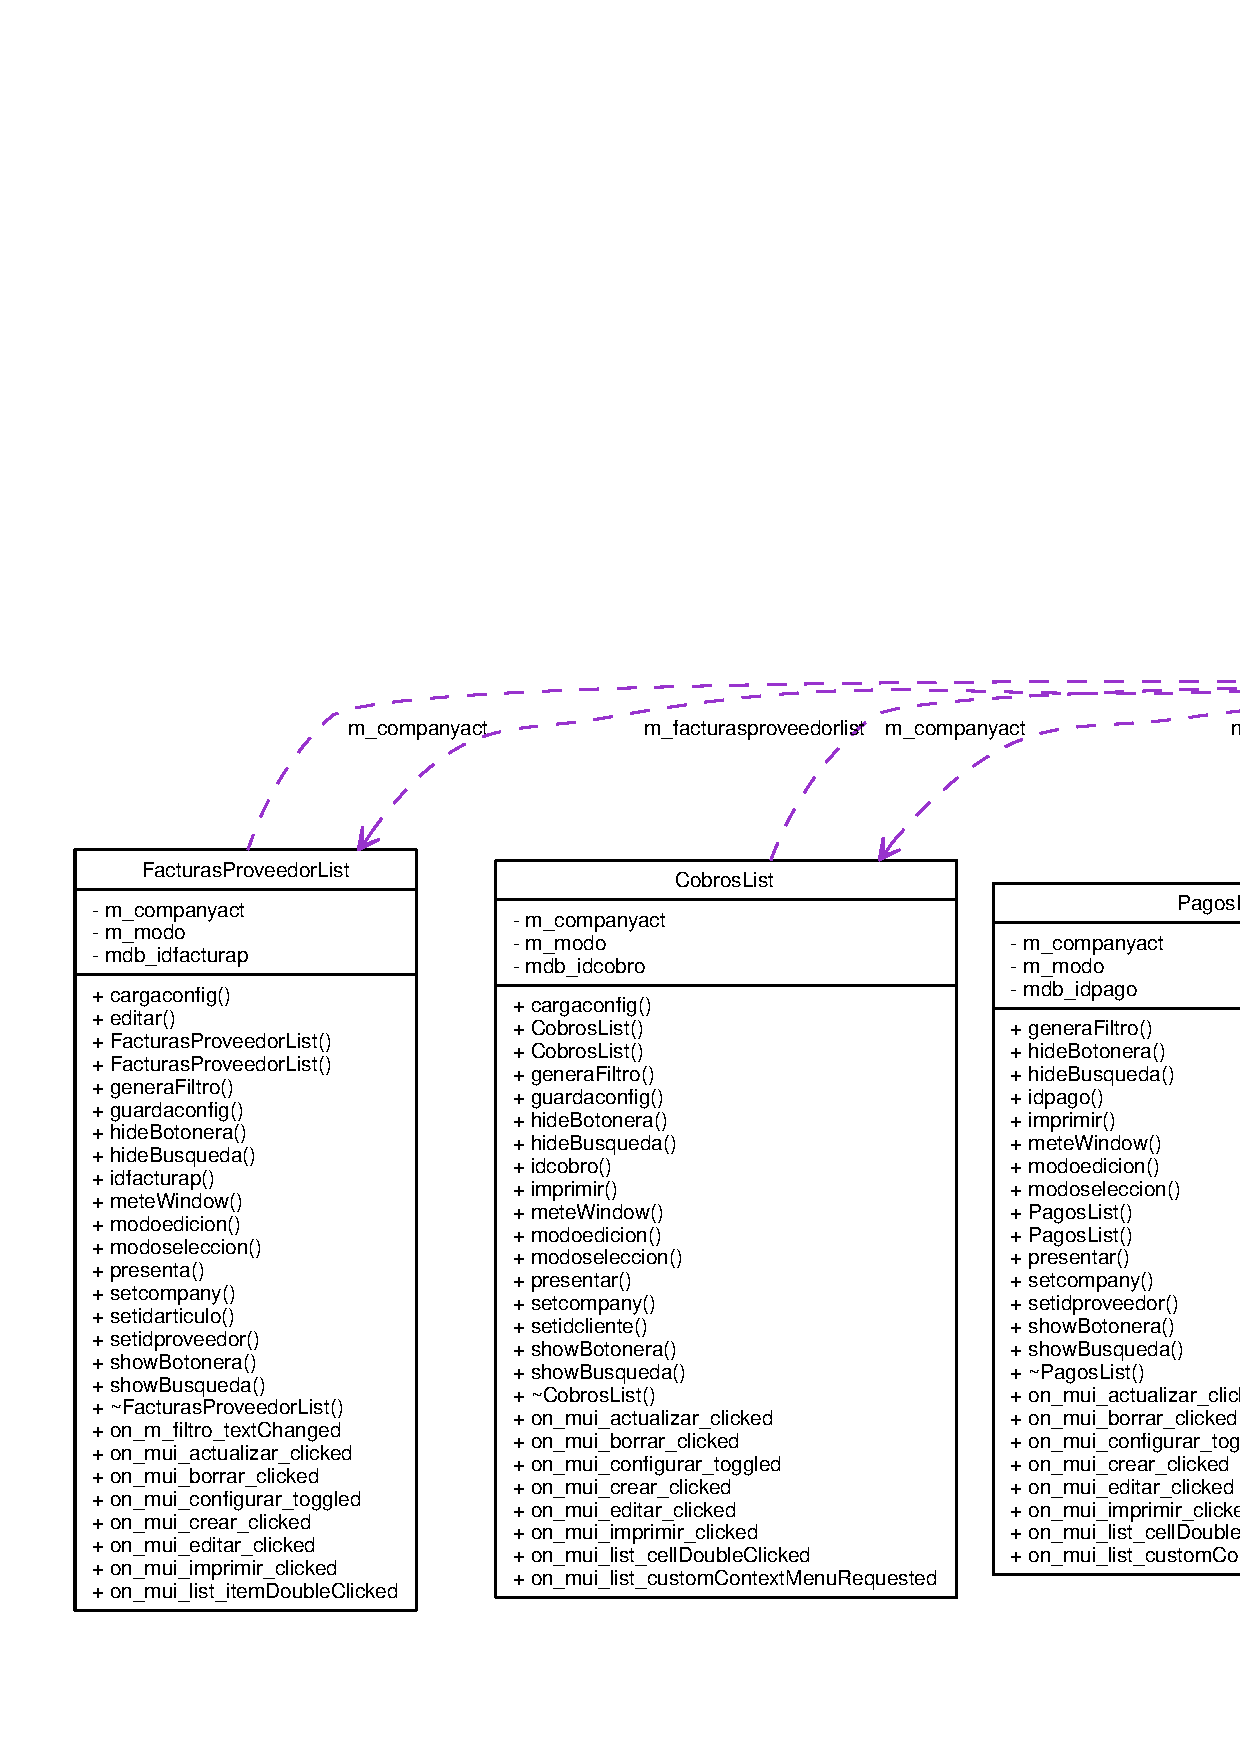
\includegraphics[width=420pt]{classcompany__coll__graph}
\end{center}
\end{figure}
\subsection*{M\'{e}todos p\'{u}blicos}
\begin{CompactItemize}
\item 
{\bf company} ()\label{classcompany_a0}

\begin{CompactList}\small\item\em El constructor de la clase company no hace nada. \item\end{CompactList}\item 
void {\bf create\-Main\-Windows} ()\label{classcompany_a1}

\item 
void {\bf init} (QString)
\item 
void {\bf l\-Albaranes\-Proveedor} ()\label{classcompany_a3}

\item 
void {\bf listarticles} ()\label{classcompany_a4}

\item 
void {\bf list\-Budgets} ()\label{classcompany_a5}

\item 
void {\bf list\-Client\-Deliv\-Notes} ()\label{classcompany_a6}

\item 
void {\bf list\-Clients} ()\label{classcompany_a7}

\item 
void {\bf listorders} ()\label{classcompany_a8}

\item 
void {\bf listproviders} ()\label{classcompany_a9}

\item 
int {\bf mete\-Window} (QString nom, QObject $\ast$obj, bool compdup=TRUE)\label{classcompany_a10}

\item 
{\bf Albaran\-Cliente\-View} $\ast$ {\bf new\-Albaran\-Cliente\-View} ()
\item 
{\bf Albaran\-Proveedor\-View} $\ast$ {\bf new\-Albaran\-Proveedor\-View} ()
\item 
{\bf Articulo\-View} $\ast$ {\bf new\-Articulo\-View} ()
\item 
{\bf Presupuesto\-View} $\ast$ {\bf new\-Budget} ()
\item 
void {\bf new\-Client\-Deliv\-Note} ()\label{classcompany_a15}

\item 
{\bf Cliente\-View} $\ast$ {\bf new\-Cliente\-View} ()
\item 
{\bf Cobro\-View} $\ast$ {\bf new\-Cobro\-View} ()\label{classcompany_a17}

\item 
{\bf Factura\-Proveedor\-View} $\ast$ {\bf new\-Factura\-Proveedor\-View} ()
\item 
{\bf Factura\-View} $\ast$ {\bf new\-Factura\-View} ()
\item 
{\bf familiasview} $\ast$ {\bf newfamiliasview} (QWidget $\ast$parent=0, bool modo\-Consulta=FALSE)
\item 
{\bf Pago\-View} $\ast$ {\bf new\-Pago\-View} ()
\item 
void {\bf new\-Pedido\-Cliente} ()\label{classcompany_a22}

\item 
{\bf Pedido\-Cliente\-View} $\ast$ {\bf new\-Pedido\-Cliente\-View} ()
\item 
{\bf Pedido\-Proveedor\-View} $\ast$ {\bf new\-Pedido\-Proveedor\-View} ()
\item 
{\bf Proveedor\-View} $\ast$ {\bf new\-Proveedor\-View} ()
\item 
{\bf Tipo\-Articulo\-List} $\ast$ {\bf new\-Tipo\-Articulo\-List} (QWidget $\ast$parent=0, bool modo\-Consulta=FALSE)
\item 
void {\bf refresh\-Albaranes\-Cliente} ()\label{classcompany_a27}

\item 
void {\bf refresh\-Albaranes\-Proveedor} ()\label{classcompany_a28}

\item 
void {\bf refresh\-Articles} ()\label{classcompany_a29}

\item 
void {\bf refresh\-Budgets} ()\label{classcompany_a30}

\item 
void {\bf refresh\-Client\-Deliv\-Notes} ()\label{classcompany_a31}

\item 
void {\bf refresh\-Clientes} ()\label{classcompany_a32}

\item 
void {\bf refresh\-Facturas} ()\label{classcompany_a33}

\item 
void {\bf refresh\-Facturas\-Proveedor} ()\label{classcompany_a34}

\item 
void {\bf refresh\-Pedidos\-Cliente} ()\label{classcompany_a35}

\item 
void {\bf refresh\-Pedidos\-Proveedor} ()\label{classcompany_a36}

\item 
void {\bf s\_\-almacenes} ()\label{classcompany_a37}

\item 
void {\bf s\_\-Familias} ()\label{classcompany_a38}

\item 
void {\bf s\_\-FPago} ()\label{classcompany_a39}

\begin{CompactList}\small\item\em Presenta la ventana de formas de pago y espera la ejecucion de la misma. \item\end{CompactList}\item 
void {\bf s\_\-indexador\-Cambia\-Estado} ()\label{classcompany_a40}

\item 
void {\bf s\_\-inventarios} ()\label{classcompany_a41}

\item 
void {\bf s\_\-list\-Facturas\-Cli} ()\label{classcompany_a42}

\item 
void {\bf s\_\-list\-Facturas\-Pro} ()\label{classcompany_a43}

\item 
void {\bf s\_\-list\-Pedidos\-Cli} ()\label{classcompany_a44}

\item 
void {\bf s\_\-list\-Pedidos\-Pro} ()\label{classcompany_a45}

\item 
void {\bf s\_\-new\-Albaran\-Cliente\-View} ()\label{classcompany_a46}

\item 
void {\bf s\_\-new\-Albaran\-Pro} ()\label{classcompany_a47}

\item 
void {\bf s\_\-new\-Albaran\-Proveedor\-View} ()\label{classcompany_a48}

\item 
void {\bf s\_\-new\-Articulo} ()\label{classcompany_a49}

\item 
void {\bf s\_\-new\-Cliente\-View} ()\label{classcompany_a50}

\item 
void {\bf s\_\-new\-Cobro\-View} ()\label{classcompany_a51}

\item 
void {\bf s\_\-new\-Factura\-Cli} ()
\item 
void {\bf s\_\-new\-Factura\-Pro} ()\label{classcompany_a53}

\item 
void {\bf s\_\-newfamiliasview} ()\label{classcompany_a54}

\item 
void {\bf s\_\-new\-Inventario} ()\label{classcompany_a55}

\item 
void {\bf s\_\-new\-List\-Configuracion\-View} ()\label{classcompany_a56}

\item 
void {\bf s\_\-new\-Pago\-View} ()\label{classcompany_a57}

\item 
void {\bf s\_\-new\-Pedido\-Cliente\-View} ()\label{classcompany_a58}

\item 
void {\bf s\_\-new\-Pedido\-Pro} ()\label{classcompany_a59}

\item 
void {\bf s\_\-new\-Pedido\-Proveedor\-View} ()\label{classcompany_a60}

\item 
void {\bf s\_\-new\-Presupuesto\-Cli} ()
\item 
void {\bf s\_\-new\-Proveedor\-View} ()\label{classcompany_a62}

\item 
void {\bf s\_\-new\-Tipo\-Articulo\-List} ()\label{classcompany_a63}

\item 
void {\bf s\_\-provincias} ()\label{classcompany_a64}

\item 
void {\bf s\_\-series\-Factura} ()\label{classcompany_a65}

\item 
void {\bf s\_\-trabajadores} ()\label{classcompany_a66}

\item 
void {\bf saca\-Window} (QObject $\ast$nom)\label{classcompany_a67}

\item 
QString {\bf search\-Company} ()
\item 
void {\bf set\-List\-Ventanas} (listventanas $\ast$doc)\label{classcompany_a69}

\item 
void {\bf set\-Workspace} (QWorkspace2 $\ast$qw)\label{classcompany_a70}

\item 
void {\bf view\-Cobros\-List} ()\label{classcompany_a71}

\item 
void {\bf view\-Pagos\-List} ()\label{classcompany_a72}

\item 
{\bf $\sim$company} ()
\begin{CompactList}\small\item\em El destructor de la clase company borra toda la memoria almacenada. \item\end{CompactList}\end{CompactItemize}
\subsection*{Atributos p\'{u}blicos}
\begin{CompactItemize}
\item 
QWorkspace2 $\ast$ {\bf m\_\-p\-Workspace}\label{classcompany_o0}

\end{CompactItemize}


\subsection{Descripci\'{o}n detallada}
Clase company (empresa). 

Clase principal del programa donde se almacenan y gestionan todos los datos de la empresa con la que se est\'{a} trabajando. 



\subsection{Documentaci\'{o}n del constructor y destructor}
\index{company@{company}!~company@{$\sim$company}}
\index{~company@{$\sim$company}!company@{company}}
\subsubsection{\setlength{\rightskip}{0pt plus 5cm}company::$\sim$company ()}\label{classcompany_a73}


El destructor de la clase company borra toda la memoria almacenada. 

Primero cerramos todas las ventanas y las Destructive\-Close se borran

Borramos el resto de ventanas. 

\subsection{Documentaci\'{o}n de las funciones miembro}
\index{company@{company}!init@{init}}
\index{init@{init}!company@{company}}
\subsubsection{\setlength{\rightskip}{0pt plus 5cm}void company::init (QString {\em bd})}\label{classcompany_a2}


Inicializa la base de datos que se pasa, si se pasa una cadena vacia entonces aparece el selector de empresa. \index{company@{company}!newAlbaranClienteView@{newAlbaranClienteView}}
\index{newAlbaranClienteView@{newAlbaranClienteView}!company@{company}}
\subsubsection{\setlength{\rightskip}{0pt plus 5cm}{\bf Albaran\-Cliente\-View} $\ast$ company::new\-Albaran\-Cliente\-View ()}\label{classcompany_a11}


Lanzamos los plugins necesarios. \index{company@{company}!newAlbaranProveedorView@{newAlbaranProveedorView}}
\index{newAlbaranProveedorView@{newAlbaranProveedorView}!company@{company}}
\subsubsection{\setlength{\rightskip}{0pt plus 5cm}{\bf Albaran\-Proveedor\-View} $\ast$ company::new\-Albaran\-Proveedor\-View ()}\label{classcompany_a12}


Lanzamos los plugins necesarios. \index{company@{company}!newArticuloView@{newArticuloView}}
\index{newArticuloView@{newArticuloView}!company@{company}}
\subsubsection{\setlength{\rightskip}{0pt plus 5cm}{\bf Articulo\-View} $\ast$ company::new\-Articulo\-View ()}\label{classcompany_a13}


Lanzamos los plugins necesarios. \index{company@{company}!newBudget@{newBudget}}
\index{newBudget@{newBudget}!company@{company}}
\subsubsection{\setlength{\rightskip}{0pt plus 5cm}{\bf Presupuesto\-View} $\ast$ company::new\-Budget ()}\label{classcompany_a14}


Lanzamos los plugins necesarios. \index{company@{company}!newClienteView@{newClienteView}}
\index{newClienteView@{newClienteView}!company@{company}}
\subsubsection{\setlength{\rightskip}{0pt plus 5cm}{\bf Cliente\-View} $\ast$ company::new\-Cliente\-View ()}\label{classcompany_a16}


Lanzamos los plugins necesarios. \index{company@{company}!newFacturaProveedorView@{newFacturaProveedorView}}
\index{newFacturaProveedorView@{newFacturaProveedorView}!company@{company}}
\subsubsection{\setlength{\rightskip}{0pt plus 5cm}{\bf Factura\-Proveedor\-View} $\ast$ company::new\-Factura\-Proveedor\-View ()}\label{classcompany_a18}


Lanzamos los plugins necesarios. \index{company@{company}!newFacturaView@{newFacturaView}}
\index{newFacturaView@{newFacturaView}!company@{company}}
\subsubsection{\setlength{\rightskip}{0pt plus 5cm}{\bf Factura\-View} $\ast$ company::new\-Factura\-View ()}\label{classcompany_a19}


Lanzamos los plugins necesarios. \index{company@{company}!newfamiliasview@{newfamiliasview}}
\index{newfamiliasview@{newfamiliasview}!company@{company}}
\subsubsection{\setlength{\rightskip}{0pt plus 5cm}{\bf familiasview} $\ast$ company::newfamiliasview (QWidget $\ast$ {\em parent} = {\tt 0}, bool {\em modo\-Consulta} = {\tt FALSE})}\label{classcompany_a20}


Lanzamos los plugins necesarios. \index{company@{company}!newPagoView@{newPagoView}}
\index{newPagoView@{newPagoView}!company@{company}}
\subsubsection{\setlength{\rightskip}{0pt plus 5cm}{\bf Pago\-View} $\ast$ company::new\-Pago\-View ()}\label{classcompany_a21}


Lanzamos los plugins necesarios. \index{company@{company}!newPedidoClienteView@{newPedidoClienteView}}
\index{newPedidoClienteView@{newPedidoClienteView}!company@{company}}
\subsubsection{\setlength{\rightskip}{0pt plus 5cm}{\bf Pedido\-Cliente\-View} $\ast$ company::new\-Pedido\-Cliente\-View ()}\label{classcompany_a23}


Lanzamos los plugins necesarios. \index{company@{company}!newPedidoProveedorView@{newPedidoProveedorView}}
\index{newPedidoProveedorView@{newPedidoProveedorView}!company@{company}}
\subsubsection{\setlength{\rightskip}{0pt plus 5cm}{\bf Pedido\-Proveedor\-View} $\ast$ company::new\-Pedido\-Proveedor\-View ()}\label{classcompany_a24}


Lanzamos los plugins necesarios. \index{company@{company}!newProveedorView@{newProveedorView}}
\index{newProveedorView@{newProveedorView}!company@{company}}
\subsubsection{\setlength{\rightskip}{0pt plus 5cm}{\bf Proveedor\-View} $\ast$ company::new\-Proveedor\-View ()}\label{classcompany_a25}


Lanzamos los plugins necesarios. \index{company@{company}!newTipoArticuloList@{newTipoArticuloList}}
\index{newTipoArticuloList@{newTipoArticuloList}!company@{company}}
\subsubsection{\setlength{\rightskip}{0pt plus 5cm}{\bf Tipo\-Articulo\-List} $\ast$ company::new\-Tipo\-Articulo\-List (QWidget $\ast$ {\em parent} = {\tt 0}, bool {\em modo\-Consulta} = {\tt FALSE})}\label{classcompany_a26}


Lanzamos los plugins necesarios. \index{company@{company}!s_newFacturaCli@{s\_\-newFacturaCli}}
\index{s_newFacturaCli@{s\_\-newFacturaCli}!company@{company}}
\subsubsection{\setlength{\rightskip}{0pt plus 5cm}void company::s\_\-new\-Factura\-Cli ()}\label{classcompany_a52}


Lanzamos los plugins necesarios. \index{company@{company}!s_newPresupuestoCli@{s\_\-newPresupuestoCli}}
\index{s_newPresupuestoCli@{s\_\-newPresupuestoCli}!company@{company}}
\subsubsection{\setlength{\rightskip}{0pt plus 5cm}void company::s\_\-new\-Presupuesto\-Cli ()}\label{classcompany_a61}


Lanzamos los plugins necesarios. \index{company@{company}!searchCompany@{searchCompany}}
\index{searchCompany@{searchCompany}!company@{company}}
\subsubsection{\setlength{\rightskip}{0pt plus 5cm}QString company::search\-Company ()}\label{classcompany_a68}


Se utiliza para mostrar un selector de empresas abreempresaview Al usuario debe seleccionar una empresa y el sistema empieza la inicializacion de clases a partir de dicha inicializacion.

El cambio de empresa se realiza desde el selector.

Si no se ha seleccionado ninguna base de datos entonces abortamos. 

La documentaci\'{o}n para esta clase fu\'{e} generada a partir de los siguientes archivos:\begin{CompactItemize}
\item 
company.h\item 
company.cpp\end{CompactItemize}
